\chapter{The Truck Backer-Upper}
% Authors: Xiao Jing,  Changgeng Zhao, 4/30/2019

In this chapter, we present the process of collecting the data, training an emulator, training the control neural net and setting the loss function. 
\section{Setup}

First we build a model of a truck basing on those kinematics:
\begin{align}
\dot x &= s \cos \theta_0 \\
\dot y &= s \sin \theta_0 \\
\dot \theta_0 &= \frac{s}{L} \tan \phi \\
\dot \theta_1 &= \frac{s}{d_1} \sin(\theta_1 - \theta_0)
\end{align}

where $s$: signed speed, $\phi$: negative steering angle, $\theta_0$: cab angle, $\theta_1$: trailer angle, $(x, y)$: position of cab. Dotted characters are the next state results of the current steering angle.

Please refer to the \href{https://github.com/Atcold/pytorch-Deep-Learning-Minicourse/blob/master/14-truck_backer-upper.ipynb}{notebook} for code details for implementing the Truck class. The basic functions of the class are: 
\begin{itemize}
\item reset: Randomly reset the initial position of the truck.
\item step: Check whether the truck is in a valid condition(not jackknifed nor off screen), then move the track backwards based on the current position and a given steering angle, according to the above equations.
\item draw: draw the parking lot and the ``cab-trailer'' to give an interactive interface of the game. The interface is shown in Figure \ref{fig:truck-interface}.
\end{itemize}

\begin{figure}[H]
    \centering
    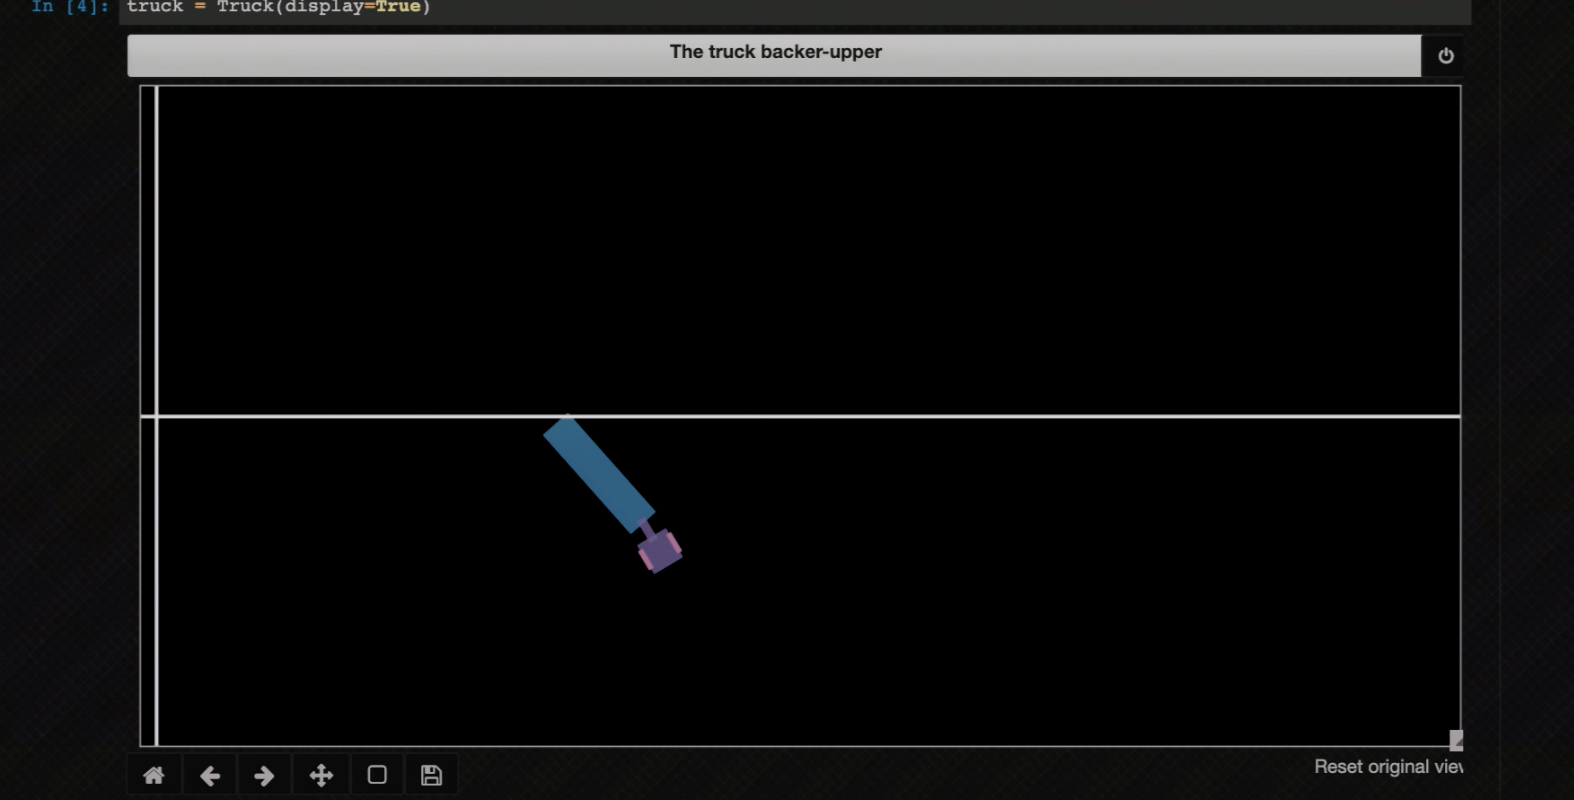
\includegraphics[width=0.7\textwidth]{labs/13/images/Screen Shot 2019-05-03 at 2.03.51 PM.png}
    \caption{The interactive interface of the truck game. A player can set the angle of the front wheels
    \label{fig:truck-interface}
    of the truck at each step.}
\end{figure}

\section{Collect Data}
In this section of the code, we generate training data for \textbf{Emulator} by randomly initializing the game and randomly steering the truck until it reaches an invalid state(jackknifes or hits the wall). We hope that this random dataset can help the \textbf{Emulator} learn the kinematics of the car.

\begin{minted}{python}
episodes = 10
data_set = list()
truck = Truck();

for episode in tqdm(range(episodes)):
    
    truck.reset()
    states = list()
    
    while truck.valid():
        ϕ = (random() - 0.5) * π / 2
        states.append((ϕ, *truck.step(ϕ)))
        truck.draw()
    
    data_set.append(states)
\end{minted}

\section{Emulator Network}
The \textbf{Emulator} is simply a 2-layer fully connected network. The input is the 6-tuple state position as well as the steering angle, and the output is the 6-tuple position of the next state. We use 45 hidden units in this particular case.

\begin{minted}{python}
state_size = 6
steering_size = 1
hidden_units_e = 45

emulator = nn.Sequential(
    nn.Linear(steering_size + state_size, hidden_units_e),
    nn.ReLU(),
    nn.Linear(hidden_units_e, state_size)
)
\end{minted}

\section{Train the emulator}

We use MSE loss and train the model state by state. Each sample in the training set is composed of the current state(input) and the next state(output).

\begin{minted}{python}
i = 0
for episode in range(len(train_set)):
    episode_loss = 0
    for _ in range(len(train_set[episode]) - 1):
        ϕ_state = train_data[i]
        next_state_prediction = emulator(ϕ_state)
        
        next_state = train_data[i + 1, 1:]
        loss = criterion(next_state_prediction, next_state)
        episode_loss += loss.item()
        
        optimiser_e.zero_grad()
        loss.backward()
        optimiser_e.step()
        i += 1
    
    # Skip end, because there is no next_frame
    i += 1
    
    if (episode + 1) % 1000 == 0 or episode == 0:
        print(f'{episode + 1:4d} / {len(train_set)}, {episode_loss:.10f}')


\end{minted}

\section{Test the emulator}
After training the emulator, we can do evaluation on the test set, which is generated by the same method as training set.

\begin{minted}{python}
i = 0
total_loss = 0
with torch.no_grad():
    for episode in range(len(test_set)):
        for _ in range(len(test_set[episode]) - 1):
            ϕ_state = test_data[i]
            next_state_prediction = emulator(ϕ_state)

            next_state = train_data[i + 1, 1:]
            total_loss += criterion(next_state_prediction, next_state).item()

            i += 1

        # Skip end, because there is no next_frame
        i += 1
    
print(f'Test loss: {loss.item():.10f}')
\end{minted}

\section{Controller Net}
The Controller Net is defined in Section~\ref{sec:truck-model} of this book and you can find it in the original paper ~\cite{nguyen1990truck}. If you can finish the remaining part of the controller network and make it work, you can \href{https://github.com/Atcold/pytorch-Deep-Learning-Minicourse/blob/master/14-truck_backer-upper.ipynb}{submit a pull request}! 